% !TeX program = xelatex
\documentclass[10pt,handout]{beamer}

\usetheme{metropolis}

\usepackage{pgfplots}
\usepgfplotslibrary{fillbetween}
\usepackage{pgfopts}
\usepackage{amsmath}
\usepackage{structuralanalysis}
\usepackage{tikz}
\usepackage{tikz-3dplot}
\usepackage{chngcntr}
\usepackage{wasysym}
\usepackage{mathtools}
\usepackage{alphalph}
\usepackage{xcolor}

\newcommand{\highlight}[1]{%
	\colorbox{red!50}{$\displaystyle#1$}}

\setcounter{lecture}{5}
\counterwithin{equation}{lecture}
\makeatletter
\def\user@resume{resume}
\def\user@intermezzo{intermezzo}
%
\newcounter{previousequation}
\newcounter{lastsubequation}
\newcounter{savedparentequation}
\setcounter{savedparentequation}{1}
% 
\renewenvironment{subequations}[1][]{%
	\def\user@decides{#1}%
	\setcounter{previousequation}{\value{equation}}%
	\ifx\user@decides\user@resume 
	\setcounter{equation}{\value{savedparentequation}}%
	\else  
	\ifx\user@decides\user@intermezzo
	\refstepcounter{equation}%
	\else
	\setcounter{lastsubequation}{0}%
	\refstepcounter{equation}%
	\fi\fi
	\protected@edef\theHparentequation{%
		\@ifundefined {theHequation}\theequation \theHequation}%
	\protected@edef\theparentequation{\theequation}%
	\setcounter{parentequation}{\value{equation}}%
	\ifx\user@decides\user@resume 
	\setcounter{equation}{\value{lastsubequation}}%
	\else
	\setcounter{equation}{0}%
	\fi
	\def\theequation  {\theparentequation  \alph{equation}}%
	\def\theHequation {\theHparentequation \alph{equation}}%
	\ignorespaces
}{%
%  \arabic{equation};\arabic{savedparentequation};\arabic{lastsubequation}
\ifx\user@decides\user@resume
\setcounter{lastsubequation}{\value{equation}}%
\setcounter{equation}{\value{previousequation}}%
\else
\ifx\user@decides\user@intermezzo
\setcounter{equation}{\value{parentequation}}%
\else
\setcounter{lastsubequation}{\value{equation}}%
\setcounter{savedparentequation}{\value{parentequation}}%
\setcounter{equation}{\value{parentequation}}%
\fi\fi
%  \arabic{equation};\arabic{savedparentequation};\arabic{lastsubequation}
\ignorespacesafterend
}
\makeatother
\title{AE 737 - Mechanics of Damage Tolerance}
\subtitle{Lecture \arabic{lecture}}
\date{Last Updated: \today}
\author{Dr. Nicholas Smith}
\institute{Wichita State University, Department of Aerospace Engineering}
% \titlegraphic{\hfill\includegraphics[height=1.5cm]{logo/logo}}

\begin{document}

\maketitle
\begin{frame}{comments}
	\begin{itemize}
		\item Superposition: addition and subtraction are fine
		\item When comparing stress intensity factors, it is important for crack length to be the same
		\item "Quarter circular crack" is a corner crack with $a=c$
		\item p. 51 My/I
		\item HW1 3 \& 16 $a=c$
		\item Added "last updated" to homework and title slide
		\item Homework can be turned in before class in my mail box or office
	\end{itemize}
\end{frame}

\begin{frame}{schedule}
	\begin{itemize}
		\item 4 Feb - Plastic Zone, Homework 1 Due, Homework 2 Assigned
		\item 9 Feb - Fracture Toughness, Homework 2 Due, Homework 3 Assigned
		\item 11 Feb - Fracture Toughness
		\item 16 Feb - Residual Strength, Homework 3 Due, Homework 4 Assigned
	\end{itemize}
\end{frame}

\begin{frame}
  \frametitle{outline}
  \setbeamertemplate{section in toc}[sections numbered]
  \tableofcontents[hideallsubsections]
\end{frame}

\section{plastic zone}

\begin{frame}{plastic zone}
	\begin{itemize}
		\item Previous developments assumed perfectly elastic materials
		\item Most common materials have some plasticity
		\item Any stress above the yield stress will undergo plastic deformation (no stress higher than $\sigma_y$ will be present in the material)
	\end{itemize}
\end{frame}

\begin{frame}{plastic zone}
	\begin{itemize}
		\item Plasticity helps retard crack propagation due to residual stresses
		\item After an overload, elastic regions will contract back to their undeformed shape
		\item The region which has undergone plastic deformation, however, holds its deformed shape
		\item This introduces a region of residual compressive stress near the crack tip
		\item Before the crack can propagate, a stress needs to overcome this residual stress
	\end{itemize}
\end{frame}

\begin{frame}{2D problems}
	\begin{itemize}
		\item We often simplify the full 3D elasticity equations for planar problems
		\item For very thin panels, we assume that all out-of-plane stresses are 0
		\item This is called plane stress
		\begin{subequations}
			\begin{align}
			\sigma_z &= \tau_{xz} = \tau_{zy} = 0\\
			\epsilon_x &= \frac{\sigma_x}{E} - \nu \frac{\sigma_y}{E}\\
			\epsilon_y &= -\nu \frac{\sigma_x}{E} + \frac{\sigma_y}{E}\\
			\epsilon_z &= -\nu \frac{\sigma_x}{E} - \nu \frac{\sigma_y}{E}\\
			\gamma_{xy} &= \frac{\tau_{xy}}{G}\\
			\gamma_{xz} &= \gamma_{yz} = 0
			\end{align}
		\end{subequations}
	\end{itemize}
\end{frame}

\begin{frame}{2D problems}
	\begin{itemize}
		\item When instead a panel is very thick, we assume that any strains through the thickness are small relative to other strains
		\item $\epsilon_z = \gamma_{xz} = \gamma_{yz} = 0$
		\item This is known as plane strain
		\begin{subequations}
			\begin{align}
			\epsilon_x &= \frac{\sigma_x}{E} - \nu \frac{\sigma_y}{E} - \nu \frac{\sigma_z}{E}\\
			\epsilon_y &= -\nu \frac{\sigma_x}{E} + \frac{\sigma_y}{E} - \nu \frac{\sigma_z}{E}\\
			0 &= -\nu \frac{\sigma_x}{E} - \nu \frac{\sigma_y}{E} + \frac{\sigma_z}{E}\\
			\gamma_{xy} &= \frac{\tau_{xy}}{G}\\
			\gamma_{xz} &= \gamma_{yz} = 0
			\end{align}
		\end{subequations}
	\end{itemize}
\end{frame}

\begin{frame}{Irwin's first approximation}
	\begin{itemize}
		\item If we recall the equation for opening stress ($\sigma_{y}$) near the crack tip
		\begin{equation}
		\sigma_y = \frac{K_I}{\sqrt{2\pi r}} \cos \frac{\theta}{2} \left(1+\sin \frac{\theta}{2}\sin \frac{3\theta}{2}\right) \tag{1.2}
		\end{equation}
		\item In the plane of the crack, when $\theta = 0$ we find
		\begin{equation*}
		\sigma_y = \frac{K_I}{\sqrt{2\pi r}}
		\end{equation*}
	\end{itemize}
\end{frame}

\begin{frame}{Irwin's first approximation}
	\begin{figure}
		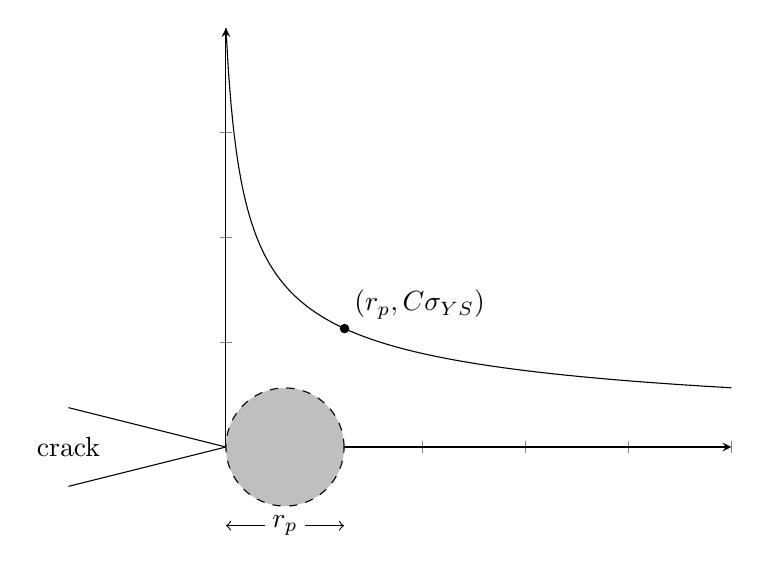
\begin{tikzpicture}
		\draw (-2,0.5) node at (-2,0) {crack} -- (0,0) -- (-2,-0.5);
		\begin{axis}[
		axis lines=middle,
		clip=false,
		ymin=0,
		xticklabels=\empty,
		yticklabels=\empty,
		cycle list name=black white,
		width=8cm,
		xmax=0.5,
		]
		\addplot+[mark=none,samples=200,unbounded coords=jump, domain=0.01:0.5] {1/sqrt(2*pi*x)};
		\draw[fill] (axis cs:0.125,1.128) circle [radius=1.5pt] node[above right] {$(r_p,C \sigma_{YS})$};
		\end{axis}
		\draw[dashed,fill=gray!50] (0.75,0) circle (0.75);
		\draw node at (0.75,-1) {$r_p$};
		\draw[->] (0.5,-1) -- (0,-1);
		\draw[->] (1,-1) -- (1.5,-1);
		\end{tikzpicture}
	\end{figure}
\end{frame}

\begin{frame}{Irwin's first approximation}
	\begin{itemize}
		\item We use $C$ "Plastic Constraint Factor" to convert between Plane Strain and Plane Stress solutions
		\item The plastic zone size can now be approximated by solving the equation $\sigma_{yy}(r=r_p) = C\sigma_{YS}$
		\pause
		\begin{subequations}
		\begin{align}
		\sigma_{yy}(r=r_p) &= C\sigma_{YS}\\
		\frac{K_I}{\sqrt{2\pi r_p}} &= C\sigma_{YS}\\
		r_p &= \frac{1}{2\pi} \left(\frac{K_I}{C\sigma_{YS}}\right)^2
		\end{align}
		\end{subequations}
	\end{itemize}
\end{frame}

\begin{frame}{Irwin's first approximation}
	\begin{itemize}
		\item For plane stress (thin panels) we let $C=1$ and find $r_p$ as
		\begin{equation}
		r_p = \frac{1}{2\pi} \left(\frac{K_I}{\sigma_{YS}}\right)^2
		\end{equation}
		\pause
		\item And for plane strain (thick panels) we let $C=\sqrt{3}$ and find
		\begin{equation}
		r_p = \frac{1}{6\pi} \left(\frac{K_I}{\sigma_{YS}}\right)^2
		\end{equation}
	\end{itemize}
\end{frame}

\begin{frame}{Intermediate panels}
	\begin{itemize}
		\item For panels which lie between plane strain and plane stress states, we use the following expression to estimate the plastic zone size
		\begin{equation}
		r_p = \frac{1}{I\pi} \left(\frac{K_I}{\sigma_{YS}}\right)^2
		\end{equation}
		\pause
		\item Where $I$ is defined as
		\begin{equation}
		I = 6.7 - \frac{1.5}{t}\left(\frac{K_I}{\sigma_{YS}}\right)^2
		\end{equation}
		\item And $2 \le I \le 6$
	\end{itemize}
\end{frame}

\begin{frame}{Irwin's second approximation}
	\begin{itemize}
		\item If our material is perfectly elastic-plastic, no stresses above $C\sigma_{YS}$ will exist in the material
		\item This ignores the strain energy (represented by the area under the curve) in the plastic zone
	\end{itemize}
\end{frame}

\begin{frame}{Irwin's second approximation}
	\begin{figure}
		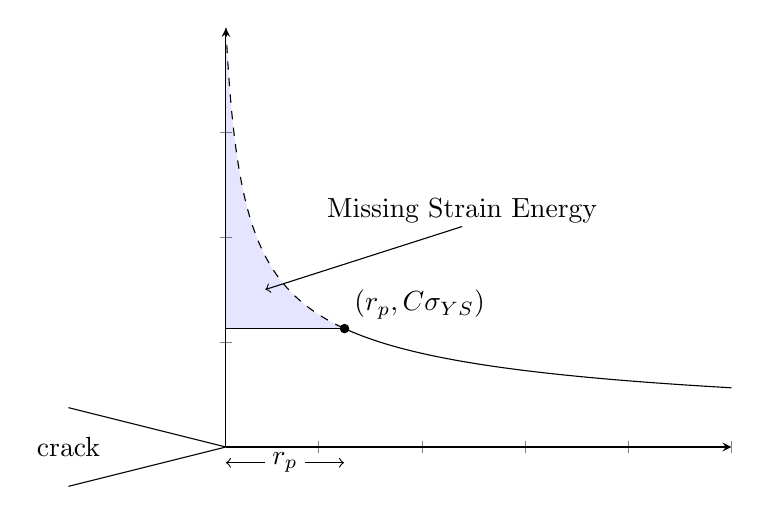
\begin{tikzpicture}
		\draw (-2,0.5) node at (-2,0) {crack} -- (0,0) -- (-2,-0.5);
		\begin{axis}[
		axis lines=middle,
		clip=false,
		ymin=0,
		xticklabels=\empty,
		yticklabels=\empty,
		cycle list name=black white,
		width=8cm,
		xmax=0.5,
		]
		\addplot[mark=none,samples=200,unbounded coords=jump, domain=0.125:0.5] {1/sqrt(2*pi*x)};
		\addplot[name path=a,mark=none,dashed,samples=200,unbounded coords=jump, domain=0.01:0.125] {1/sqrt(2*pi*x)};
		\addplot[name path=b,mark=none,samples=200,unbounded coords=jump, domain=0.01:0.125] {1/sqrt(2*pi*.125)};
		\addplot[fill=blue, fill opacity=.1] fill between[of=a and b];
		\draw[fill] (axis cs:0.125,1.128) circle [radius=1.5pt] node[above right] {$(r_p,C \sigma_{YS})$};
		\end{axis}
		\draw node at (0.75,-.2) {$r_p$};
		\draw[->] (0.5,-.2) -- (0,-.2);
		\draw[->] (1,-.2) -- (1.5,-.2);
		\draw node at (3,3) {Missing Strain Energy};
		\draw[->] (3,2.8) -- (0.5,2);
		\end{tikzpicture}
	\end{figure}
\end{frame}

\begin{frame}{Irwin's second approximation}
	\begin{itemize}
		\item To account for the additional strain energy, Irwin considered a plastic zone size increased by some $\delta$
		\item He also needed to adjust the stress function, and considered an equivalent crack tip in these calculations
	\end{itemize}
\end{frame}

\begin{frame}{Irwin's second approximation}
	\begin{figure}
		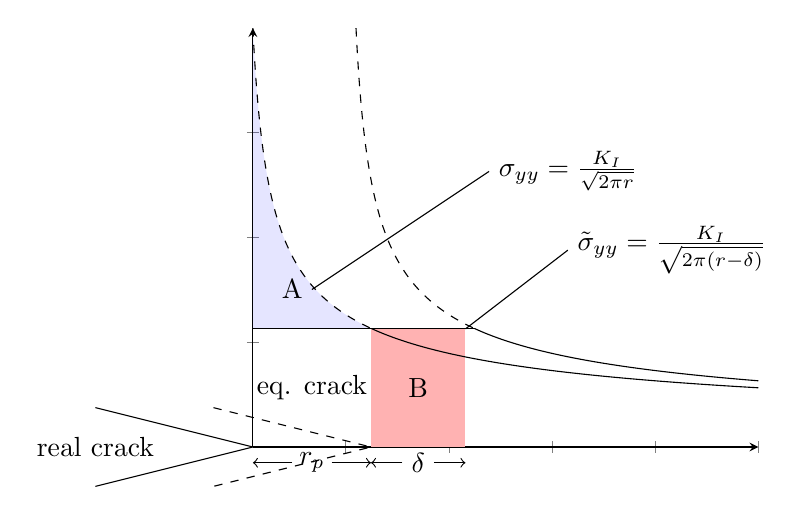
\begin{tikzpicture}
		\draw (-2,0.5) node at (-2,0) {real crack} -- (0,0) -- (-2,-0.5);
		\draw[dashed] (-.5,0.5) node at (.75,.75) {eq. crack} -- (1.5,0) -- (-.5,-0.5);
		\fill[red!30] (1.5,0) rectangle (2.7,1.5);
		\begin{axis}[
		axis lines=middle,
		clip=false,
		ymin=0,
		xticklabels=\empty,
		yticklabels=\empty,
		cycle list name=black white,
		width=8cm,
		xmax=0.5,
		]
		\addplot[mark=none,samples=200,unbounded coords=jump, domain=0.125:0.5] {1/sqrt(2*pi*x)};
		\addplot[name path=a,mark=none,dashed,samples=200,unbounded coords=jump, domain=0.01:0.125] {1/sqrt(2*pi*x)};
		\addplot[name path=b,mark=none,samples=200,unbounded coords=jump, domain=0.01:0.225] {1/sqrt(2*pi*.125)};
		\addplot[fill=blue, fill opacity=.1] fill between[of=a and b];
		\addplot[name path=c,mark=none,dashed,samples=200,unbounded coords=jump, domain=0.11:0.225] {1/sqrt(2*pi*(x-.1))};
		\addplot[name path=d,mark=none,samples=200,unbounded coords=jump, domain=0.225:0.5] {1/sqrt(2*pi*(x-.1))};
		\end{axis}
		\draw node at (0.75,-.2) {$r_p$};
		\draw[->] (0.5,-.2) -- (0,-.2);
		\draw[->] (1,-.2) -- (1.5,-.2);
		\draw node at (2.1,-.2) {$\delta$};
		\draw[->] (2.3,-.2) -- (2.7,-.2);
		\draw[->] (1.9,-.2) -- (1.5,-.2);
		\draw[-] (3,3.5) node[right] {$\sigma_{yy} = \frac{K_I}{\sqrt{2\pi r}}$} -- (0.75,2);
		\draw[-] (4,2.5) node[right] {$\tilde{\sigma}_{yy} = \frac{K_I}{\sqrt{2\pi (r-\delta)}}$} -- (2.7,1.5);
		\draw node at (.5,2) {A};
		\draw node at (2.1,0.75) {B};
		\end{tikzpicture}
	\end{figure}
\end{frame}

\begin{frame}{Irwin's second approximation}
	\begin{itemize}
		\item We need $A=B$, so we set them equivalent and solve for $\delta$.
		\begin{subequations}
			\begin{align}
			A &= \int_{0}^{r_p} \sigma_{yy} dr - r_p \sigma_{YS}\\
			&= \int_{0}^{r_p} \frac{K_I}{\sqrt{2\pi r}} dr - r_p \sigma_{YS}\\
			&= \frac{K_I}{\sqrt{2\pi}}\int_{0}^{r_p} r^{-1/2} dr - r_p \sigma_{YS}\\
			&= \frac{2K_I \sqrt{r_p}}{\sqrt{2\pi}}- r_p \sigma_{YS}
			\end{align}
		\item We have already found $r_p$ as
		\begin{equation}
		r_p = \frac{1}{2\pi} \left(\frac{K_I}{\sigma_{YS}}\right)^2
		\end{equation}
		\item If we solve this for $K_I$ we find
		\begin{equation}
		K_I = \sqrt{2\pi r_p} \sigma_{YS}
		\end{equation}
		\end{subequations}
	\end{itemize}
\end{frame}

\begin{frame}{Irwin's second approximation}
	\begin{itemize}
		\item We can now substitute back into the strain energy of A
		\begin{subequations}[resume]
			\begin{align}
			A &= \frac{2\sqrt{2\pi r_p} \sigma_{YS} \sqrt{r_p}}{\sqrt{2\pi}}- r_p \sigma_{YS}\\
			&= 2 \sigma_{YS} r_p- r_p \sigma_{YS}\\
			&= r_p \sigma_{YS}
			\end{align}
		\item B is given simply as $B = \delta \sigma_{YS}$, so we equate A and B to find $\delta$
		\begin{align}
		A &= B\\
		r_p \sigma_{YS} &= \delta \sigma_{YS}\\
		r_p &= \delta
		\end{align}
		\end{subequations}
	\end{itemize}
\end{frame}

\begin{frame}{Irwin's second approximation}
	\begin{itemize}
		\item This means the plastic zone size is simply $2r_p$
		\item However, it also means that the effective crack length is $a + r_p$
		\pause
		\item Since $r_p$ depends on $K_I$, we must iterate a bit to find the "real" $r_p$ and $K_I$
	\end{itemize}
\end{frame}

\begin{frame}{Example}
	\begin{figure}[H]
		\centering
		\begin{tikzpicture}
		\draw (0,0) -- (0,2) -- (4,2) -- (4,-2) -- (0,-2) -- (0,0);
		\draw (0,0) -- (0.5,0);
		\draw node at (0.75,0.2) {a};
		\draw[->] (2,2) -- (2,2.5) node[above] {$\sigma$};
		\draw[->] (2,-2)-- (2,-2.5) node[below] {$\sigma$};
		\draw[->] (1.5,-0.5) -- (0,-0.5);
		\draw[->] (2.5,-0.5) -- (4,-0.5);
		\draw node at (2,-0.5) {$W$};
		\end{tikzpicture}
	\end{figure}
\end{frame}

\begin{frame}{equations}
	\begin{align}
	\beta &= \left[1.122 - 0.231 \frac{a}{W} + 10.55 \left(\frac{a}{W}\right)^2 - 21.71 \left(\frac{a}{W}\right)^3 + 30.82 \left(\frac{a}{W}\right)^4\right] \tag{2.4a}\\
	I &= 6.7 - \frac{1.5}{t}\left(\frac{K_I}{\sigma_{YS}}\right)^2 \tag{4.13}\\
	r_p &= \frac{1}{I\pi} \left(\frac{K_I}{\sigma_{YS}}\right)^2 \tag{4.12}
	\end{align} 
\end{frame}

\section{plastic stress intensity ratio}

\begin{frame}{plastic stress intensity ratio}
\begin{itemize}
\item Engineers often use stress intensity to decide which material to use for a certain application
\item The ratio of plastic stress intensity to elastic stress intensity, as a function of yield stress over applied stress, can help illustrate the effects of plasticity for different materials.
\end{itemize}
\end{frame}

\begin{frame}{plastic stress intensity ratio}
	\begin{itemize}
		\item For an infinitely wide center-cracked panel, we can solve for $K_{Ie}/K_I$ symbolically
		\item For plane stress we have:
		\begin{subequations}
			\begin{align}
			K_I &= \sigma \sqrt{\pi a}\\
			K_{Ie} &= \sigma \sqrt{\pi(a+r_p)}\\
			r_p &= \frac{1}{2\pi} \left( \frac{K_{Ie}}{\sigma_{YS}}\right)^2\\
			K_{Ie} &= \sigma \sqrt{\pi \left(a+\frac{1}{2\pi} \left( \frac{K_{Ie}}{\sigma_{YS}}\right)^2\right)}
			\end{align}
		\end{subequations}
	\end{itemize}
\end{frame}

\begin{frame}{plastic stress intensity ratio}
	\begin{itemize}
		\item We square both sides
		\begin{subequations}[resume]
			\begin{align}
			K_{Ie}^2 &= \sigma^2 \pi \left(a+\frac{1}{2\pi} \left( \frac{K_{Ie}}{\sigma_{YS}}\right)^2\right)\\
			K_{Ie}^2 &= \sigma^2 \pi a+\frac{\sigma^2}{2} \left( \frac{K_{Ie}}{\sigma_{YS}}\right)^2\\
			K_{Ie}^2 - \frac{\sigma^2}{2} \left( \frac{K_{Ie}}{\sigma_{YS}}\right)^2 &= \sigma^2 \pi a\\
			K_{Ie}^2\left(1 - \frac{\sigma^2}{2 \sigma_{YS}^2}\right) &= \sigma^2 \pi a
			\end{align}
		\end{subequations}
	\end{itemize}
\end{frame}

\begin{frame}{plastic stress intensity ratio}
	\begin{itemize}
		\item We divide both sides by $\left(1 - \frac{\sigma^2}{2 \sigma_{YS}^2}\right)$
		\begin{subequations}[resume]
			\begin{align}
			K_{Ie}^2 &= \frac{\sigma^2 \pi a}{1 - \frac{\sigma^2}{2 \sigma_{YS}^2}}\\
			K_{Ie} &= \frac{\sigma \sqrt{\pi a}}{\sqrt{1 - \frac{\sigma^2}{2 \sigma_{YS}^2}}}\\
			K_{Ie} &= \frac{K_I}{\sqrt{1 - \frac{\sigma^2}{2 \sigma_{YS}^2}}}\\
			\frac{K_{Ie}}{K_I} &= \frac{1}{\sqrt{1 - \frac{\sigma^2}{2 \sigma_{YS}^2}}}
			\end{align}
		\end{subequations}
	\end{itemize}
\end{frame}

\begin{frame}{plastic stress intensity ratio}
	\begin{itemize}
		\item We can also find the plastic stress intensity ratio numerically for finite width panels
		\item Panel thickness, yield stress, panel width, crack length could all be variables in this case
		\item Different heat treatments of metal alloys can give a different yield stress, with most other properties remaining the same
		\item Typical crack lengths can vary based on inspection cycles
	\end{itemize}
\end{frame}

\begin{frame}{example}
	\begin{itemize}
		\item You are trying to design an appropriate inspection cycle on a panel
		\item One item to consider is the plastic stress intensity ratio, consider the effect of varying crack lengths on the plastic stress intensity ratio.
		\begin{figure}[H]
			\centering
			\begin{tikzpicture}
			\begin{scope}[scale=.5]
			\draw (0,-3) -- (0,3) -- (6,3) -- (6,-3) -- (0,-3);
			\draw[->] (3,3) -- (3,4) node[above] {8 ksi};
			\draw[->] (3,-3) -- (3,-4) node[below] {8 ksi};
			\draw (0,0) -- (2,0);
			\draw node at (1.2,0.5) {$a$};
			\draw[->] (2.5,-2.5) -- (0,-2.5);
			\draw[->] (3.5,-2.5) -- (6,-2.5);
			\draw node at (3,-2.5) {5"};
			\end{scope}
			\end{tikzpicture}
		\end{figure}
	\end{itemize}
\end{frame}

\section{plastic zone shape}

\begin{frame}{plastic zone shape}
\begin{itemize}
\item Although we drew a circle to give a rough idea of the plastic zone in Irwin's method, this solution was only 1D
\item We considered $\theta=0$.
\item It is advantageous to model the plastic zone shape, we will do so using two different yield theories
\item Von Mises and Tresca
\end{itemize}
\end{frame}

\begin{frame}{principal stresses}
	\begin{itemize}
		\item Principal stresses are often used in yield theories
		\item We can determine the principal stresses near the crack tip as
		\begin{subequations}
			\begin{align}
			\label{eq:principal}
			\sigma_1 &= \frac{K_I}{\sqrt{2\pi r}}\cos \frac{\theta}{2}\left(1+\sin \frac{\theta}{2}\right)&\\
			\sigma_2 &= \frac{K_I}{\sqrt{2\pi r}}\cos \frac{\theta}{2}\left(1-\sin \frac{\theta}{2}\right)&\\
			\sigma_3 &= 0 &\qquad \text{(plane stress)}\\
			\sigma_3 &= \frac{2\nu K_I}{\sqrt{2\pi r}}\cos \frac{\theta}{2} &\qquad \text{(plane strain)}
			\end{align}
		\end{subequations}
	\end{itemize}
\end{frame}

\begin{frame}{Von Mises yield theory}
\begin{itemize}
\item The Von Mises yield theory is also known as the Distortion Energy Yield Theory
\item In this yield theory, we assume that failure or yielding occurs when the strain energy exceeds some threshold
\item It has been observed that hydrostatic pressure does not generally cause yielding
\item We separate the strain energy into two parts, volumetric and distortional
\item Only the distortional strain energy is used to determine the yield strength
\end{itemize}
\end{frame}

\begin{frame}{Von Mises yield theory}
	\begin{itemize}
		\item The distortional strain energy is given by
		\begin{equation}
		\label{eq:distortion}
		W_d = \frac{1}{12}G\left[\left(\sigma_1 - \sigma_2\right)^2 + \left(\sigma_2 - \sigma_3\right)^2 + \left(\sigma_3 - \sigma_1\right)^2\right]
		\end{equation}
		\item Which for a uniaxially loaded point becomes
		\begin{equation}
		W_d = \frac{1}{6}G\sigma_{YS}^2
		\end{equation}
		\item We can equate the two cases and solve
		\begin{subequations}
			\begin{align}
			\frac{1}{6}G\sigma_{YS}^2 &= \frac{1}{12}G\left[\left(\sigma_1 - \sigma_2\right)^2 + \left(\sigma_2 - \sigma_3\right)^2 + \left(\sigma_3 - \sigma_1\right)^2\right]\\
			2 \sigma_{YS}^2 &= \left(\sigma_1 - \sigma_2\right)^2 + \left(\sigma_2 - \sigma_3\right)^2 + \left(\sigma_3 - \sigma_1\right)^2
			\end{align}
		\end{subequations}
	\end{itemize}
\end{frame}

\begin{frame}{Von Mises yield theory}
	\begin{itemize}
		\item We can find the plastic zone size, $r_p$ by substituting the principal stress relations (\ref{eq:principal}) into the distortional strain energy equation (\ref{eq:distortion})
		\item In plane stress we find
		\begin{subequations}
			\begin{align}
			2 \sigma_{YS}^2 &= \left( \sigma_1 - \sigma_2 \right)^2 + \left( \sigma_2 - 0 \right)^2 + \left(0 - \sigma_1\right)^2\\
			&\begin{aligned}
			\mathllap{2 \sigma_{YS}^2} &= \left(\frac{K_I}{\sqrt{2\pi r_p}}\cos \frac{\theta}{2}\left(1+\sin \frac{\theta}{2}\right) - \frac{K_I}{\sqrt{2\pi r_p}}\cos \frac{\theta}{2}\left(1-\sin \frac{\theta}{2}\right)\right)^2 + \\
			&\qquad \left(\frac{K_I}{\sqrt{2\pi r_p}}\cos \frac{\theta}{2}\left(1-\sin \frac{\theta}{2}\right) - 0\right)^2 + \\
			&\qquad \left(0 - \frac{K_I}{\sqrt{2\pi r_p}}\cos \frac{\theta}{2}\left(1+\sin \frac{\theta}{2}\right)\right)^2
			\end{aligned}
			\end{align}
		\end{subequations}
	\end{itemize}
\end{frame}

\begin{frame}{Von Mises yield theory}
	\begin{itemize}
		\item After solving we find
		\begin{equation}
			r_p = \frac{K_I^2}{2\pi \sigma^2_{YS}} \cos^2 \frac{\theta}{2} \left(1 + 3\sin^2 \frac{\theta}{2}\right)
		\end{equation}
		\item We can similarly solve for $r_p$ in plane strain to find
		\begin{equation}
		r_p = \frac{K_I^2}{2\pi \sigma^2_{YS}} \cos^2 \frac{\theta}{2} \left(1 -4\nu + 4\nu^2 + 3\sin^2 \frac{\theta}{2}\right)
		\end{equation}
	\end{itemize}
\end{frame}

\begin{frame}{Tresca yield theory}
	\begin{itemize}
		\item Tresca yield theory assumes that yielding begins when the maximum shear stress reaches a critical value
		\item In uniaxial tension this gives
		\begin{equation}
		\tau_0 = \tau_{max} = \frac{1}{2}\left(\sigma_{max} - \sigma_{min}\right) = \frac{1}{2} \left(\sigma_{YS} - 0\right) = \frac{\sigma_{YS}}{2}
		\end{equation}
	\end{itemize}
\end{frame}

\begin{frame}{Tresca yield theory}
	\begin{itemize}
		\item Using (\ref{eq:principal}), we see that 
		\begin{subequations}
			\begin{align}
			\sigma_{max} &= \frac{K_I}{\sqrt{2\pi r}}\cos \frac{\theta}{2}\left(1+\sin \frac{\theta}{2}\right)\\
			\sigma_{min} &= 0
			\end{align}
		\end{subequations}
		\item We can substitute and solve as before to find
		\begin{equation}
		r_p = \frac{K_I^2}{2 \pi \sigma_{YS}^2}\cos^2 \frac{\theta}{2}\left(1+\sin \frac{\theta}{2}\right)^2
		\end{equation}
	\end{itemize}
\end{frame}

\begin{frame}{Tresca yield theory}
	\begin{itemize}
		\item In plane strain, it is not clear whether $\sigma_2$ or $\sigma_3$ will be $\sigma_{min}$
		\item We can solve for when $\sigma_2$ will be $\sigma_{min}$
		\begin{subequations}
			\begin{align}
			\sigma_2 &< \sigma_3\\
			\frac{K_I}{\sqrt{2\pi r}}\cos \frac{\theta}{2}\left(1-\sin \frac{\theta}{2}\right) &< \frac{2\nu K_I}{\sqrt{2\pi r}}\cos \frac{\theta}{2}\\
			1-\sin \frac{\theta}{2} &< 2\nu\\
			\theta_t > 2 \sin^{-1} (1-2\nu)
			\end{align}
		\end{subequations}
	\end{itemize}
\end{frame}

\begin{frame}{Tresca yield theory}
	\begin{itemize}
		\item When $2\pi - \theta_t < \theta < \theta_t$, $\sigma_2$ is the minimum, otherwise $\sigma_3$ is the minimum
		\item Note: Error(s) in text p. 101
		\item Once we have chosen the appropriate minimum stress ($\sigma_2 or \sigma_3$), we can solve for $r_p$ as before
	\end{itemize}
\end{frame}

\begin{frame}{Tresca yield theory}
	\begin{subequations}
		\begin{align}
		r_p &= \frac{2 K_I^2}{\pi \sigma_{YS}^2} \cos^2 \frac{\theta}{2} \sin^2 \frac{\theta}{2} & \theta_t < \theta < 2\pi - \theta_t\\
		r_p &= \frac{K_I^2}{2\pi \sigma_{YS}^2}\cos^2 \frac{\theta}{2}\left(1 - 2\nu + \sin \frac{\theta}{2}\right)^2 & \theta < \theta_t, \theta > 2\pi - \theta_t
		\end{align}
	\end{subequations}
\end{frame}

\begin{frame}{3D plastic zone shape}
	
\begin{figure}
\centering
\includegraphics[width=0.7\linewidth]{dumbell}
\label{fig:dumbell}
\end{figure}
\end{frame}
\end{document}
